%%%%%%%%%%%%%%%%%%%%%%%%%%%%%%%%%%%%%%%%%%%%%%%%%%%%%%%%%%%%%%%%%%%%%
%
%  This is a sample LaTeX input file for your contribution to
%  the PHYSOR2018 topical meeting.
%
%  Please use it as a template for your full paper
%    Accompanying/related file(s) include:
%       1. Document class/format file: physor2018.cls
%       2. Sample Postscript Figure:   figure.pdf
%       3. A PDF file showing the desired appearance: physor2018_template.pdf
%       4. cites.sty and citesort.sty that might be needed by some users
%    Direct questions about these files to: rcarlos.lope@gmail.com
%											armando.gomez@inin.gob.mx
%
%    Notes:
%      (1) You can use the "dvips" utility to convert .dvi
%          files to PostScript.  Then, use either Acrobat
%          Distiller or "ps2pdf" to convert to PDF format.
%      (2) Different versions of LaTeX have been observed to
%          shift the page down, causing improper margins.
%          If this occurs, adjust the "topmargin" value in the
%          physor2018.cls file to achieve the proper margins.
%
%%%%%%%%%%%%%%%%%%%%%%%%%%%%%%%%%%%%%%%%%%%%%%%%%%%%%%%%%%%%%%%%%%%%%


%%%%%%%%%%%%%%%%%%%%%%%%%%%%%%%%%%%%%%%%%%%%%%%%%%%%%%%%%%%%%%%%%%%%%
\documentclass[letterpaper]{physor2018}
%
%  various packages that you may wish to activate for usage
\usepackage{tabls}
\usepackage{cites}
\usepackage{epsf}
\usepackage{appendix}
\usepackage{ragged2e}
\usepackage[top=1in, bottom=1.in, left=1.in, right=1.in]{geometry}
\usepackage{enumitem}
\usepackage{subcaption}
\setlist[itemize]{leftmargin=*}
\usepackage{caption}
\captionsetup{width=1.0\textwidth,font={bf,normalsize},skip=0.3cm,within=none,justification=centering}
\usepackage[per-mode=symbol,inter-unit-product={}\cdot{},bracket-unit-denominator=false]{siunitx}
\usepackage{microtype}

%\usepackage[justification=centering]{caption}

%
% Define title...
%
\title{PRELIMINARY COUPLING OF OpenMC AND Nek5000\\
WITHIN THE MOOSE FRAMEWORK}
%
% ...and authors
%
\author{%
  % FIRST AUTHORS
  %
  \textbf{A. Novak$^{1}$, P. Romano$^2$, B. Wendt$^3$, R. Rahaman$^2$, E. Merzari$^2$,}\\
  \textbf{L. Kerby$^{3,4}$, C. Permann$^4$, R. Martineau$^4$, and R.N. Slaybaugh$^{1}$}\\
  \\
  $^1$University of California-Berkeley\\
  3115 Etcheverry Hall, Berkeley, CA 94708\\
\\
  $^2$Argonne National Laboratory\\ 
    9700 S. Cass Avenue, Lemont, IL 60439\\ 
     \\
 $^3$Department of Nuclear Engineering, Idaho State University \\
      921 South 8\textsuperscript{th} Avenue, Pocatello, ID 83209\\
     \\
  $^4$Idaho National Laboratory\\
  2525 Fremont Avenue, Idaho Falls, ID 83402\\
     \\
  \url{novak@berkeley.edu}, \url{promano@anl.gov}, \url{wendbryc@isu.edu}
}
%
% Insert authors' names and short version of title in lines below
%
\newcommand{\authorHead}      % Author's names here use et al. if more than 3
           {April Novak et al.}
\newcommand{\shortTitle}      % Short title here (Shorten to fit all into a single line)
           {Preliminary Coupling of OpenMC and Nek5000}
%%%%%%%%%%%%%%%%%%%%%%%%%%%%%%%%%%%%%%%%%%%%%%%%%%%%%%%%%%%%%%%%%%%%%
%
%   BEGIN DOCUMENT
%
%%%%%%%%%%%%%%%%%%%%%%%%%%%%%%%%%%%%%%%%%%%%%%%%%%%%%%%%%%%%%%%%%%%%%
\begin{document}
\maketitle
\justify

\begin{abstract}
This paper presents a Monte Carlo-computational fluid dynamics coupling of OpenMC
and Nek5000 within the MOOSE framework. This coupling specifically
aims to address and overcome challenges encountered in earlier coupling works
such as file-based communication and overly restrictive one-to-one mesh mappings
between the codes. In addition, coupling within the MOOSE framework offers
the possibility of relatively easy coupling to any other MOOSE application. The
advantages of the coupling framework are illustrated with a simple pincell example;
to demonstrate the ease of coupling to other MOOSE applications,
a lightweight surrogate for BISON, called Buffalo, is used to solve for the nuclear fuel physics.
\end{abstract}
\keywords{Monte Carlo, CFD, thermal-hydraulics, MOOSE}

\section{INTRODUCTION}
With the continual improvement in computing resources, it is becoming
increasingly feasible to employ Monte Carlo (MC) and thermal-hydraulics (T/H)
tools for coupled analysis of nuclear systems. Nuclear systems exhibit feedback
between neutron transport and thermal-hydraulics through the
temperature dependence of nuclear data and the energy released from nuclear
reactions. For systems with a thermal neutron spectrum, the two strongest
feedback mechanisms are
  1)~Doppler feedback, whereby an increase in fuel temperature causes cross
  sections to broaden, increasing parasitic absorption,
  and 2)~moderator density feedback, whereby a decrease in moderator density
  causes a reduction in moderation.
Establishing these feedback mechanisms is often
critical to ensuring a stable reactor.

With continuous-energy and continuous-angle physics and flexible geometry descriptions, MC
codes have long been the highest-fidelity tools to solve the neutron transport
equation. Computational fluid dynamics (CFD) codes, with fewer fundamental
assumptions regarding the models used for aspects such as momentum transfer and
turbulence, are frequently used to capture high-resolution flow details.
Coupled MC-CFD simulations permit high-resolution and geometrically complex
models of reactor behavior, which can improve understanding of complicated
systems such as fluid-fueled reactors and the first wall of fusion reactors. In
addition, such tools provide robust benchmarking capabilities.  Many authors
have developed software that couples single-physics MC and T/H codes
together~\cite{Wu,Seker,Cardoni,Breitkreutz,Sjenitzer,Gurecky,Ivanov,Daeubler,Aufiero,Gill}. Here we
present the coupling of OpenMC, an open source MC code~\cite{Romano}, and
Nek5000, an open source CFD code~\cite{Fischer}, within the Multiphysics Object Oriented
Simulation Environment (MOOSE) finite element framework~\cite{Gaston}.
Section~\ref{sec:first} discusses the software design and overall coupling
structure; Section~\ref{sec:Representation} the data transfer between codes;
Section~\ref{sec:Results} the results for a simple test problem; and
Section~\ref{sec:Conclusions} the many next steps in improving the coupling
design.

\section{SOFTWARE DESIGN}
\label{sec:first}

Generally, two software design methods are used for coupling single-physics codes,
each of which has unique advantages and challenges.
The majority of previous MC-T/H couplings utilized
an external coupling paradigm, where the flow of execution is controlled with a specially developed script.
This script coordinates data exchange by performing input/output (I/O) on files specific to each code.
For each Picard step, this script alternately runs MC and T/H solutions,
parsing output files and rewriting input files to achieve data transfers.
Examples of external coupling include
Serpent and RELAP5~\cite{Wu}, MCNP5 and STAR-CCM+~\cite{Cardoni},
MCNPX and CFX~\cite{Breitkreutz}, MCNP6 and FLUENT~\cite{Gurecky}, and
TRIPOLI and SUBCHANFLOW~\cite{Sjenitzer}.
External coupling is required if accessing the source code directly is not possible.
Filesystem-based I/O can become a bottleneck for large problems,
and the scripts developed often have low potential for reuse in other coupling applications
because they are highly specific to each code's file formats.
Continually editing a 200,000\(+\) line input file for large
problems while simultaneously updating a source file after each iteration to improve convergence
should be avoided if possible~\cite{Ivanov}.

Alternatively, codes can be coupled at a source code level via the internal
coupling paradigm by making the changes needed to pass information in memory,
rather than through the filesystem.  OpenMC and Nek5000 can be internally
coupled by using OpenMC as the driver and inserting calls to Nek5000 routines
where needed (or vice versa) or by using a driver that calls both OpenMC and
Nek5000 routines. This driver could be developed from scratch or OpenMC and
Nek5000 melded to the structure of an existing driver.  While internal coupling
has not been the predominant MC-T/H coupling method, several recent couplings
such as Serpent 2 with SUBCHANFLOW~\cite{Daeubler} and OpenFOAM~\cite{Aufiero}
and MC21 with CTF~\cite{Gill} have been performed.  In the present work, an internal
coupling between OpenMC and Nek5000 was achieved using the MOOSE framework as
the driver.  While internal coupling generally requires more development work
and access to source code, the coupling is agnostic to input file structure and
provides the opportunity to make simultaneous code algorithmic changes and reuse
the coupling interface.

Previous work by Ellis et al.~\cite{Ellis} involved the coupling of OpenMC and MOOSE, but because of
design changes in the data transfers and coupling structure and a lack of access to the project code,
the coupling was performed from scratch.
This work presents the first coupling of MC and CFD codes together within
the MOOSE framework, and to our knowledge one of the first, if not the first,
MC-CFD coupling using a well-established external driver such as MOOSE.
The advantage of coupling within MOOSE is the lowered complexity
of extending the coupling of
OpenMC and/or Nek5000 to include other MOOSE applications.
To illustrate this last benefit, all of the couplings performed in this work couple OpenMC,
Nek5000, and Buffalo. Buffalo is a lightweight surrogate for BISON, a
nuclear fuels simulation code based on the MOOSE framework.
Substitution of BISON into
this coupling framework can be performed easily.

\subsection{Coupling within the MOOSE Framework}
\label{sec:MOOSECoupling}
In order to couple codes using an existing driver, the subroutines of each code must be
cast into the structure of the driver framework. The following sections discuss the
Picard iteration coupling structure and
modifications made to the OpenMC and Nek5000 source
codes to permit their coupling within the MOOSE framework.

\subsubsection{Code execution}
In order to run an external code within the MOOSE framework, its routines must
be adapted to MOOSE class methods. A transient MOOSE simulation is controlled
by the {\tt Transient} executioner class. This class defines methods that are called at the
start and end of a simulation and once per Picard iteration.
Code reorganization to fit the driver structure and compilation as a MOOSE application
is referred to in this paper as ``wrapping.''
For the present work, OpenMC is wrapped as a MOOSE application named Okapi
and Nek5000 as a MOOSE application named Giraffe.
OpenMC and Nek5000 are built as dynamic libraries to permit access
to subroutines within MOOSE.
The details of this wrapping are beyond the scope of this paper, but to illustrate the
types of changes performed, we describe the changes made to the OpenMC source to fit
into the MOOSE {\tt Transient} executioner class.
An OpenMC simulation was originally controlled by a single subroutine
that read input files, transported particles, accumulated tally results,
and printed output files. This subroutine was split into a number of smaller subroutines that
are suitable for use in the MOOSE {\tt Transient} class.
The reading of input files and memory allocation was
placed into a separate subroutine, {\tt openmc\_init}.
The transport of particles was placed into its own subroutine, {\tt openmc\_run}.
At the end of each Picard step, tallies need to be cleared so that they are not accumulated
for every iteration; a new routine {\tt openmc\_reset} performs
such cleanup activities.
At the end of the simulation, {\tt openmc\_finalize} frees memory and writes output files.
A similar procedure is performed for the Nek5000 wrapping and is not discussed here.
In addition to code restructuring to allow Picard iterations, subroutines are added or
modified to facilitate data exchange in memory; these are discussed in Section~\ref{sec:DataTransfer}.

MOOSE uses a tree-like coupling structure in which execution and data
transfer are controlled by a Master App.
Subordinate to this Master App are any number of MultiApps.
Many parallel instances of a MultiApp can
run simultaneously, representing independent solves.
Fig.~\ref{fig:MultiApps} shows the coupling hierarchy for a
coupled Okapi-Giraffe-Buffalo simulation of an assembly. Because Okapi is the
only application that solves over the entire domain, it is natural
 to select Okapi as the Master App. Because there are multiple thermally independent fuel pins,
many parallel instances of Buffalo run simultaneously.
In this preliminary work, the coupling
is only performed for a single fuel pin, but this tree
structure easily extends to full assembly calculations.
Any of the three codes may execute first provided the appropriate
initial conditions. For the present work, the order of execution in a single
Picard step is shown in Fig.~\ref{fig:Simple_Picard}.
In each time step, Nek5000, then OpenMC, then
Buffalo performs individual physics solves.
Data is exchanged between each of these solves.
After all three codes have run, convergence is evaluated;
Picard iterations are repeated
until convergence. After convergence at a time step,
Buffalo and Giraffe move to the next
time step; OpenMC runs in \(k\)-eigenvalue mode.

\begin{figure}[!htb]
  \centering
  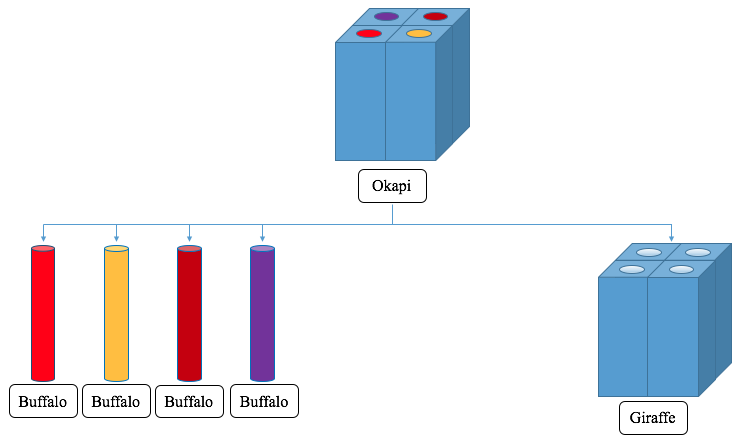
\includegraphics[scale=0.4]{../Figures/heirarchy.png}
  \caption{Coupling hierarchy for a fuel assembly simulation with Okapi solving for the neutron transport, Giraffe the fluid dynamics, and Buffalo the nuclear fuel physics.}
  \label{fig:MultiApps}
\end{figure}

\begin{figure}[!htb]
  \centering
  \includegraphics[scale=0.55]{../Figures/simple_Picard.pdf}
  \caption{Simple depiction of orders of execution in a Picard step.}
  \label{fig:Simple_Picard}
\end{figure}

% might not have space:
%OpenMC is written in Fortran 2008, Nek5000 in Fortran 77, and MOOSE in C++. MOOSE performs all calls to OpenMC and Nek5000 routines, which requires care with language interoperability. The {\tt ISO\_C\_BINDING} intrinsic module is used to allow OpenMC routines to be easily called by a C++ code. Nek5000 common blocks directly map to C++ structs, and with name mangling macros, Nek5000 routines can be easily called by a C++ code.

\subsubsection{Internal data transfer}
\label{sec:DataTransfer}
In addition to restructuring source code to permit Picard iteration,
internal coupling requires subroutines to facilitate
in-memory data transfers. The MOOSE framework defines many classes
to facilitate data transfer between libMesh-based applications,
but custom transfer classes are needed to exchange data with external codes.
A new C-language application programming interface
 is under development in OpenMC that defines
routines commonly needed for coupling, such as routines to change cell temperatures and
densities, extract tally information, and set boundary conditions (BCs).
A detailed discussion of these routines added to the OpenMC and Nek5000
source codes is outside the scope of this paper.

%%% Will it be presented somewhere else? %%%
%%% A: Maybe once it's more stable and cleaned up? %%%

The most important MC-T/H feedback effects are captured by the fission
distribution, fuel and moderator temperature, and fuel and moderator density.
All five of these data transfers have been implemented in the present work,
but in the simple test problem in Section~\ref{sec:Results}, the fuel density
is not included. Energy deposition outside the fuel is currently neglected. Fig.~\ref{fig:Simple_Picard}
shows the major steps performed in a single Picard step.
Thin arrows indicate data transfers, which are performed by using the custom transfer classes.
Bold arrows represent execution flow, controlled by the custom executioner classes.
At the start of each time step, Okapi passes a wall heat flux BC to Giraffe,
where internally the information is passed to a Nek5000 subroutine that applies this BC.
Next, Nek5000 runs a CFD simulation. The fluid temperature and density
and a fuel surface
temperature BC are transferred from Giraffe to Okapi by querying Nek5000 subroutines.
The fluid temperature and density are passed directly into OpenMC subroutines.
In this tree coupling hierarchy, Buffalo and Giraffe cannot
communicate directly, so the temperature BC is stored by Okapi
before transfer to Buffalo.
With updated fluid conditions, OpenMC runs a MC simulation.
Okapi then transfers the fission distribution by querying OpenMC subroutines and
the transfers wall temperature BC to Buffalo. Buffalo reconstructs the fission
distribution into a heat source in the fuel, then solves for temperature and density of the fuel.
Buffalo then transfers the updated fuel density and temperature to Okapi by directly calling
OpenMC subroutines, and transfers the updated wall heat flux BC to Okapi
to be stored before transfer to Giraffe at the start of the next Picard iteration.

\section{DATA REPRESENTATION}
\label{sec:Representation}
OpenMC transports particles on a constructive solid geometry model of the problem.
Strictly speaking, the number of geometry cells need only be
enough to accurately represent the geometry,
since the resolution of the solution depends
on the number of particles. On the other hand,
codes solving partial differential equations discretize these equations on a mesh,
and the resolution is directly dependent on the mesh. CFD simulations
require particularly fine meshes to capture boundary layers and
the fine-scale structures of turbulence.
The number of MC cells required to describe
typical reactor geometries is
much less than the number required for an accurate CFD or fuels simulation. This mesh disparity
makes transferring data challenging.
The choices made for data representation in the present work are described in
the following sections. In Sections
~\ref{sec:THtoMC} and ~\ref{sec:MCtoTH}, the term ``T/H'' is used
to refer to both Buffalo and Nek5000 because
in principle Nek5000 could solve for the temperature in the fuel with its
conjugate heat transfer modules. In Section~\ref{sec:FuelstoCFD}, where
the data transfer between Buffalo and Nek5000 is discussed,
the term ``T/H'' is again used to refer to the CFD solution in the fluid.

\subsection{Thermal-Hydraulics to Monte Carlo Data Transfer}
\label{sec:THtoMC}
During the transport routine, a distance to collision \(d\) is sampled by solving

\begin{equation}
  \label{DCollision}
\xi=\int_0^d\Sigma_t(x)\exp{\left(-\int_{x_0}^x\Sigma_t(x')dx'\right)}dx,
\end{equation}

where \(\xi\) is a uniformly distributed random number on the interval \([0,1]\), \(\Sigma_t\) is the total
cross section, \(x\) is the distance along the particle's current flight path,
and \(x_0\) is the particle's current position. This equation can be difficult or impossible to solve
analytically when \(\Sigma_t(x)\) is a continuous function of \(x\).
If \(\Sigma_t\) is constant, however, Eq. (\ref{DCollision}) simplifies to

\begin{equation}
\label{DCollision2}
d=\frac{-\ln{(\xi)}}{\Sigma_t}\ .
\end{equation}

Traditional surface tracking routines sample \(d\) according to Eq.~(\ref{DCollision2}).
If the distance to the next cell is closer than this distance, then the assumption of constant
\(\Sigma_t\) is no longer valid, so the particle is moved to the surface,
and the tracking process is repeated.
A T/H code computes continuous temperatures and densities. For surface-tracking-based
MC codes, this implies solution of Eq.~(\ref{DCollision}).
Instead, the majority of previous MC-T/H
couplings have opted to perform volume averaging of temperatures and densities
in the T/H code such that a homogeneous material can be applied in the corresponding
MC cell~\cite{Cardoni,Breitkreutz,Sjenitzer,Gurecky,Ivanov}.
To avoid large discretization errors, this approach sometimes necessitates
using an enormous number of MC cells.
Transporting particles on a large number of cells
involves a dramatic increase in memory to store the additional
geometry and material information
while also requiring more surface crossings,
both of which slow the calculation.
For a pincell geometry, only four cells should be needed to describe the geometry
(three concentric cylinders and the water cell).
To retain the T/H solution details for similar pin cell test
problems, Seker used 228 cells~\cite{Seker}, Cardoni 7,489 cells~\cite{Cardoni},
and Gurecky 14,776 cells~\cite{Gurecky} in the MC models.

In order to alleviate the requirement of large numbers of MC cells, a solution to Eq.~(\ref{DCollision})
using the method described in~\cite{Brown} is currently being implemented
in OpenMC.
Since this method is not yet complete,
all results shown in this paper use cell-uniform temperatures and densities in the MC geometry.
Buffalo computes a functional expansion (FE)
for the fuel temperature using
new capabilities added to the MOOSE framework that are discussed in
a companion paper~\cite{Wendt}; only the zeroth-order
term, which represents an average, is currently used in OpenMC
subroutines to change cell temperatures and
densities. Orthogonal FEs
are described in Section~\ref{sec:MCtoTH}. Because orthogonal functions are difficult
to define over the water portion
of a pincell, subroutines have been added to Nek5000 that
compute axial averages of fluid
temperature and density given a desired number of averaging layers; these averaged
values are communicated to the same OpenMC
subroutines.

Some MC codes also transport particles
using the delta-tracking approach~\cite{Leppanen}.
By introducing the concept of a virtual collision, the total cross section can
be made uniform through the geometry so that the distance to collision
is always sampled by Eq.~(\ref{DCollision2}).
At each collision, the T/H code can simply be queried as to the T/H conditions
given a particle's coordinates,
and the local \(\Sigma_t\) can be determined according to the
method chosen to form the temperature-dependent
cross sections.
Because of known disadvantages associated with delta-tracking, 
thresholds usually enforce switching between surface- and delta-tracking;
this requirement of supporting surface-tracking
does not alleviate the need to solve Eq.~(\ref{DCollision}).
Based on the efficiency of the solution to Eq.~(\ref{DCollision2}), other tracking methods may be pursued.

\subsection{Monte Carlo to Thermal-Hydraulics Data Transfer}
\label{sec:MCtoTH}
To capture a fine spatial dependence in the MC code,
either a very large number of tallies must be defined
or else a FE for the fission power distribution must be determined.
Breitkreutz reported the need to use \SI{25}{\micro\meter} tally
cells to accurately capture the fission distribution for a research reactor~\cite{Breitkreutz}.
Large numbers of tallies are associated with similar issues related to memory requirements
as using large numbers of cells. In addition, for a fixed number of particles,
a finer spatial tally mesh results in higher tally variance,
since fewer particles score to each tally.
The present work alleviates the need for a fine tally mesh by
expressing the fission power distribution \(P\)
in terms of FEs of orthogonal polynomials. For a generic 3-D expansion over a
cylinder, the fission distribution can be expressed as

\begin{equation}
P(r,\theta,z)=\sum_{l=0}^L\sum_{m=0}^M\sum_{n=0}^NC_{lmn}\psi_{lm}(r,\theta)\phi_n(z),
\end{equation}

where \(\psi_{lm}\) is a generic polynomial orthogonal on the unit circle
and \(\phi_n\) is a generic polynomial orthogonal on a Cartesian axis.
By orthogonality, the coefficients \(C_{lmn}\) are given as integral
quantities over the orthogonal domains \(\Omega\)
of the polynomials, multiplied by the fission power:

\begin{equation}
C_{lmn}=\int_{\Omega_{r,\theta}}\int_{\Omega_z}P(r,\theta,z)\psi_{lm}(r,\theta)\phi_n(z)\omega(r,\theta,z)rdrd\theta dz,
\end{equation}

where \(\omega(r,\theta,z)\) is the weighting function with respect to which the polynomials
are orthogonal. All MC tallies are integral
quantities, so an integral expression for expansion coefficients fits nicely into
the tally framework.
The benefit of FEs as opposed to one-to-one MC-T/H cell transfers
is that a relatively small number of tallies, one tally bin per coefficient,
can be used to capture a complex spatial behavior. In addition, when a particle
scores to an FE tally (FET), it scores to every tally bin. Therefore, increasing the order of the
FET does not increase the variance of existing tally bins,
although more particles are required to capture the increasingly complex
higher-order polynomial terms. A disadvantage of FETs is that orthogonal
polynomials cannot be constructed for all geometries.
FETs have recently been implemented in Serpent, and a comparison
was made with the typical histogram-type distribution used in
conventional tallies~\cite{Kerby}.
In previous work, Ellis et al. implemented Zernike polynomials, which are orthogonal on the unit circle,
in OpenMC~\cite{Ellis}. These FETs are utilized in the present work, and extension to
other functions and higher dimensions is ongoing.
The fission power distribution is tallied in the fuel pin, and only the
coefficients are transferred to Buffalo, which reconstructs a
continuous heat source using new capabilities
in the MOOSE framework~\cite{Wendt}.

\subsection{Nuclear Fuels to Thermal-Hydraulics Data Transfer}
\label{sec:FuelstoCFD}

For the present work, Buffalo and Nek5000 are coupled through the
BCs on the fuel surface.
Subroutines were added to Nek5000 to facilitate the application
of a BC given external information and calculation of the
information needed to describe a computed BC to an external code.
Due to the advantages associated with FE representations
discussed in Section~\ref{sec:MCtoTH}, FE capabilities were
implemented in Nek5000. Nek5000 computes the expansion coefficients for an
orthogonal series describing the fuel surface temperature
and transfers these coefficients to Buffalo.
Buffalo then reconstructs a continuous
BC from these coefficients. For the reverse direction, Buffalo also computes
an orthogonal FE for the fuel surface heat flux, which is
reconstructed as a continuous BC by Nek5000.
Work is ongoing in extending the FE capabilities within Nek5000.

\section{RESULTS}
\label{sec:Results}
This section presents results for a simple pincell problem. The problem setup
is intended to demonstrate feedback effects between the various physics and
should not be construed as the actual simulation of a real system.
Several simplifications are made in the
models used, since the purpose of this paper is a preliminary display of a
coupling framework. While the largest asymmetries in the fission power distribution
in light water reactors tend to occur
axially, 3-D FETs have not yet been fully implemented in
OpenMC; thus, this example is purposefully constructed to exhibit
strong radial asymmetries that can be captured by
the 2-D FETs currently available in OpenMC.
The geometry consists of two fuel pins situated side by side, but
the coupling is only performed for one pin for simplicity. In other words, while
OpenMC transports neutrons over the entire geometry, Nek5000 and Buffalo only
perform simulations of the fluid and fuel in the left pincell.
These two pins have radii of \SI{0.5}{\centi\meter} and height of \SI{1}{\centi\meter} with a pitch of \SI{0.6}{\centi\meter}.
The left pin consists of \(\textrm{UO}_2\) fuel,
while the right pin consists of boron oxide. This absorber pin represents a
strong absorber whose purpose is to skew the fission distribution
such that a skew in the fuel temperature,
fluid density, and fuel surface BCs is clearly visible.
OpenMC is used to determine the fission distribution, Nek5000 the fluid temperature
and density, and Buffalo the fuel temperature. In this example, Buffalo
solves for the fuel temperature. If kernels to solve for fuel density are included in
the Buffalo input file, then density can also be expanded in an orthogonal functional
series and its coefficients passed into OpenMC routines.
Nek5000 can solve the fully 3-D, compressible Navier-Stokes
equations. For simplicity, the transient incompressible Navier-Stokes equations are
solved here in nondimensional form for laminar flow; an equation of state
for the fluid density in terms of temperature is used to approximate compressibility.

The fission distribution is expanded in a 6th-order Zernike, zeroth-order
Legendre series using a tally of the recoverable fission energy,
for a total of 28 expansion coefficients for the pin.
OpenMC is run with 150 inactive
cycles and 800 active cycles of 100,000 particles each, giving less than \(\pm0.00006\)\
uncertainty in \(k_{\infty}\). Reflective BCs are used on all boundaries.
Nek5000 assumes a constant inlet velocity of \SI{1}{\meter\per\second} and temperature of \SI{550}{\kelvin}.
Symmetric BCs are applied on all lateral faces, no-slip
BCs on the fuel surface, and outflow BCs at the top of the pincell.
A heat flux BC computed by Buffalo is applied on the fuel surface.
Because a numerical solution to Eq. (\ref{DCollision}) is under development,
Nek5000 performs axial integration of the fluid temperature in
four layers and passes this information to the corresponding OpenMC cell.
Buffalo solves the time-dependent
heat conduction equation in the fuel with constant thermal diffusivity (\SI{1}{\meter^2/\second}).
Insulated BCs are applied on the top and bottom of
the pincell, and a Dirichlet temperature BC computed by Nek5000
on the fuel surface. The fuel surface heat flux and temperature are each expanded in
Buffalo and Nek5000 as 7th-order Fourier, 10th-order Legendre series for a total of 88
coefficients per BC. The fuel temperature
is expanded as a Zernike-Legendre series in Buffalo, but due to the ongoing
development of a numerical solution to Eq. (\ref{DCollision}), only the zeroth-order
coefficient is used in OpenMC.
The expansion orders used in this example were selected to be sufficiently large
to display the expected distribution shapes; optimization of expansion orders
for a specific problem is deferred to future work.
The initial conditions in Nek5000 set the zeroth-order heat flux
coefficient to \SI{1} and the fluid to an isothermal \SI{550}{\kelvin}. An isothermal fuel
temperature of \SI{600}{\kelvin} is set in both OpenMC and Buffalo.
Buffalo convergence is defined on a nonlinear solve relative tolerance of
\(10^{-8}\).
Coupled convergence is based on the relative change in the average fuel temperature being
less than 0.5\%, but the simulation is run beyond this limit to compensate for the
fact that more complicated convergence estimates based on multiple solution fields
are not used. The simulation is manually stopped at 12 iterations.
Fig.~\ref{fig:k_avgtmp}
shows \(k_{\infty}\) and the average fuel temperature, with their absolute
and relative change, respectively, from the previous iteration as a function of Picard iteration.
Based on the convergence criteria, the Picard iteration converges in
6 iterations. However, scatter in \(k_{\infty}\)
beyond statistical uncertainty for iterations 8 and 9 suggests
convergence criteria should also consider \(k_{\infty}\).

\begin{figure}[!htb]
\centering
\begin{subfigure}{.5\textwidth}
  \centering
  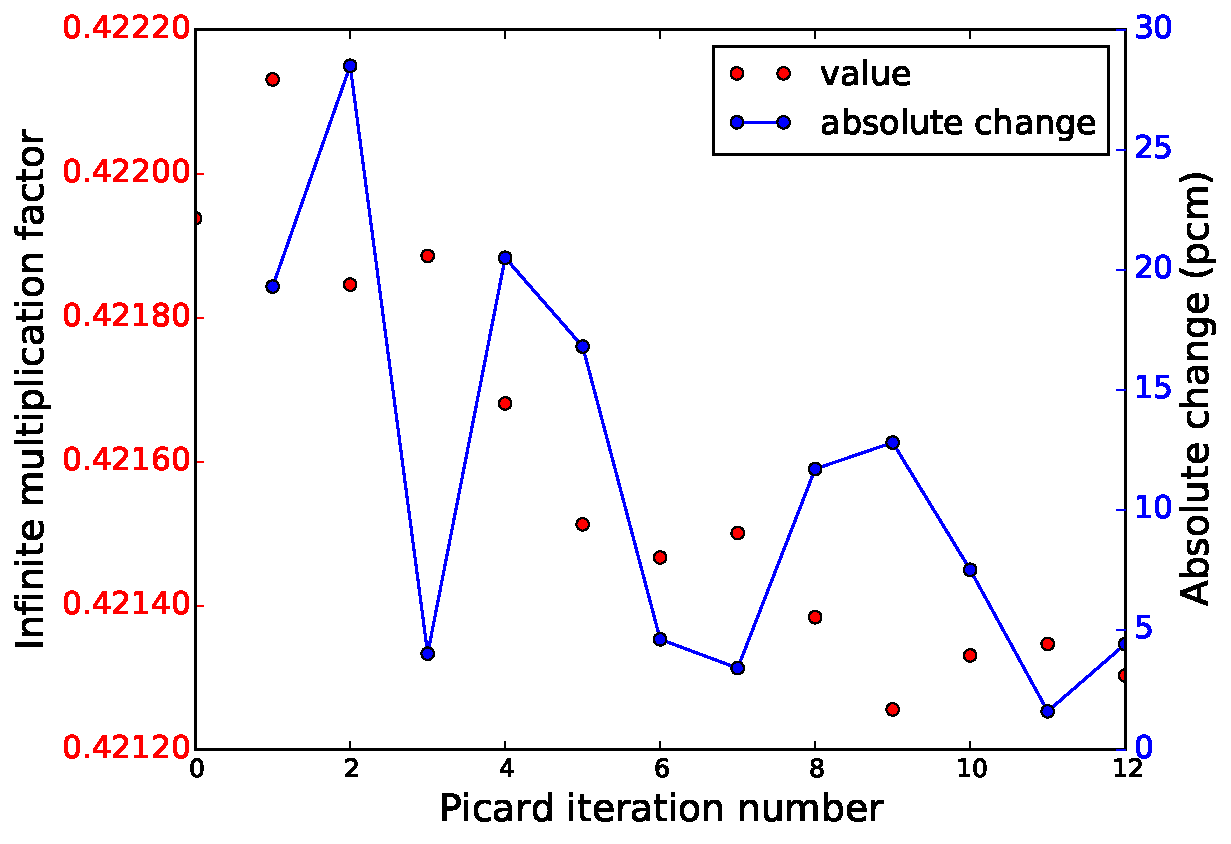
\includegraphics[width=0.75\linewidth]{../Figures/k_eff.pdf}
  \caption{\(k_{\infty}\)}
\end{subfigure}%
\begin{subfigure}{.5\textwidth}
  \centering
  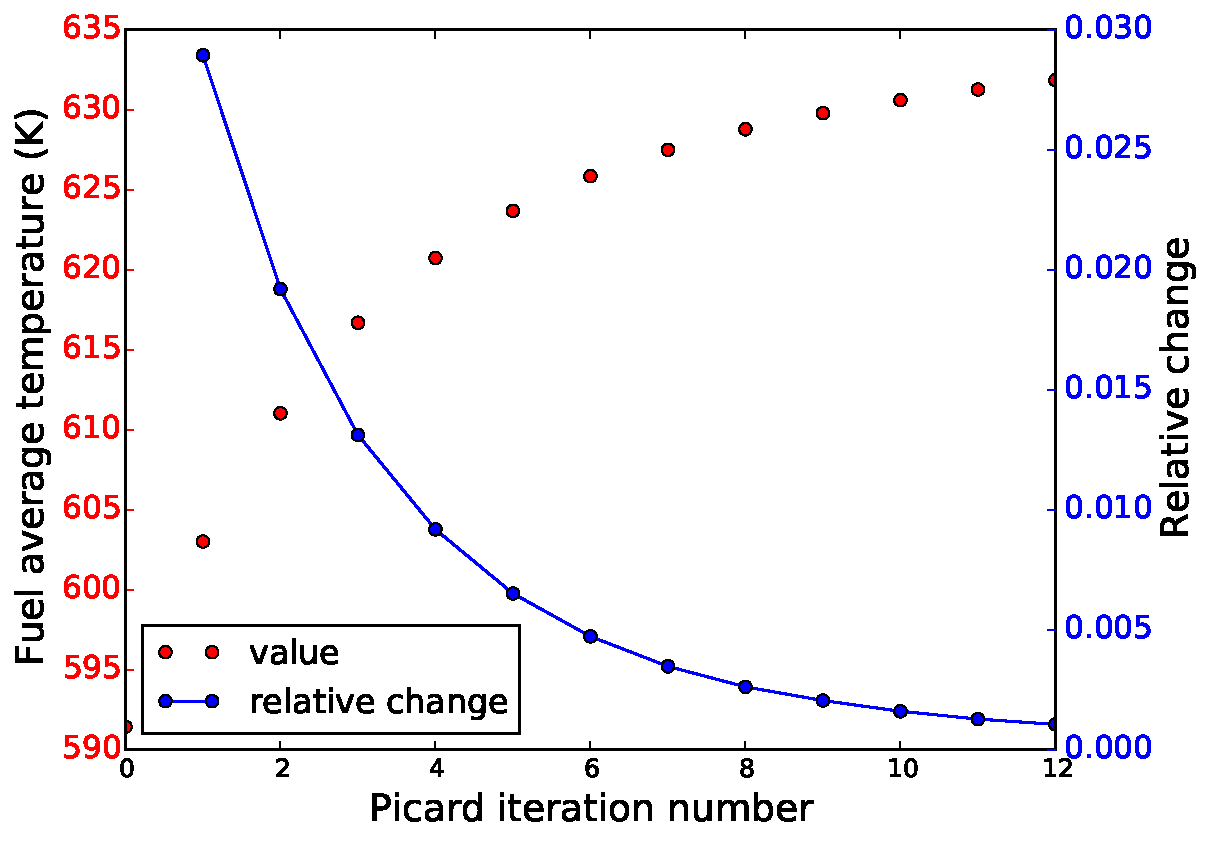
\includegraphics[width=0.75\linewidth]{../Figures/temp.pdf}
  \caption{Average fuel temperature}
\end{subfigure}
\caption{(a) \(k_{\infty}\) and (b) average
fuel temperature, with absolute and relative changes, respectively,
for the UO$_2$ fuel pin as a function of Picard iteration. The uncertainty
in \(k_{\infty}\) for each point is 0.00006.}
\label{fig:k_avgtmp}
\end{figure}

Fig.~\ref{fig:openmc_buffalo} shows the recoverable fission energy distribution
and fuel temperature
 at iteration 12 at the top of the pin. All other results in this
 paper are shown at iteration 12 as well unless otherwise noted. The presence of the
strong absorber pin to the right (not in the figure) causes the power to be significantly
lower on the right half of the pin. While more
difficult to see, the fuel temperature peak is also skewed to the left. The maximum
temperature occurs at a distance of \SI{0.035}{\centi\meter} to the left of the pin center,
showing the coupling between higher powers and higher temperatures.
With only 28 coefficients, both the fission and temperature distributions are
captured fairly well. Fig.~\ref{fig:fuel_temps} shows the fuel surface temperature
BC computed by Nek5000 for the left and right halves of the pin. The right half,
with a lower power because it faces the absorber pin, shows a lower
surface temperature BC; this can be seen by focusing
on the lightest shade in the color scale.
With only 88 coefficients, Fig.~\ref{fig:fuel_temps}
demonstrates the potential of using FEs to also pass mesh-based information.

\begin{figure}[!htb]
\centering
\begin{subfigure}{.5\textwidth}
  \centering
  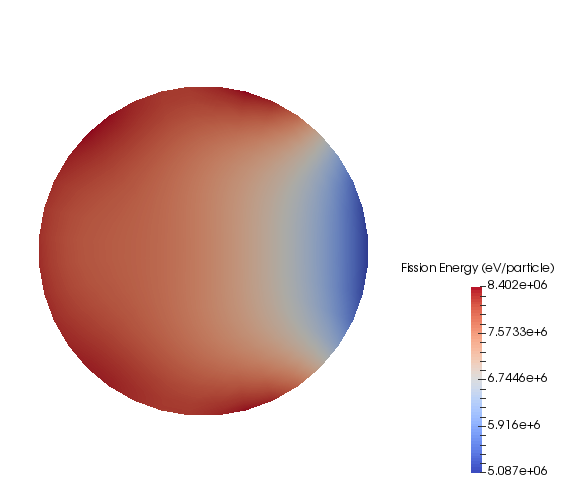
\includegraphics[width=0.75\linewidth]{../Figures/kappa_fission.png}
  \caption{Fission energy (eV/particle)}
\end{subfigure}%
\begin{subfigure}{.5\textwidth}
  \centering
  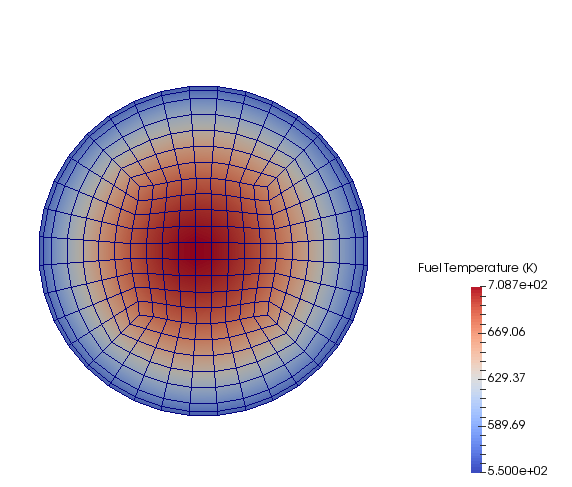
\includegraphics[width=0.75\linewidth]{../Figures/fuel_temp.png}
  \caption{Fuel temperature (K)}
\end{subfigure}
\caption{(a) Recoverable fission energy and (b)
fuel temperature for the UO$_2$ fuel pin.}
\label{fig:openmc_buffalo}
\end{figure}

\begin{figure}[!htb]
\centering
\begin{subfigure}{.5\textwidth}
  \centering
  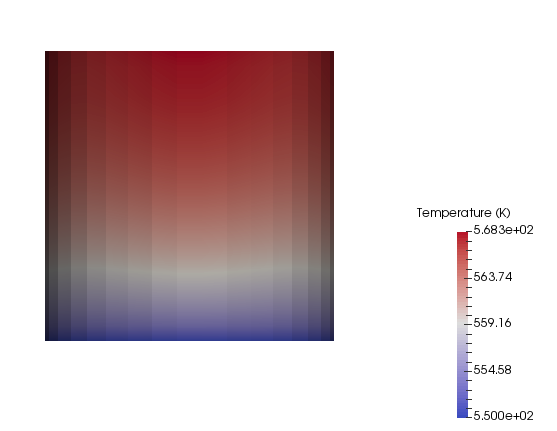
\includegraphics[width=0.8\linewidth]{../Figures/temp_left.png}
  \caption{Left side}
\end{subfigure}%
\begin{subfigure}{.5\textwidth}
  \centering
  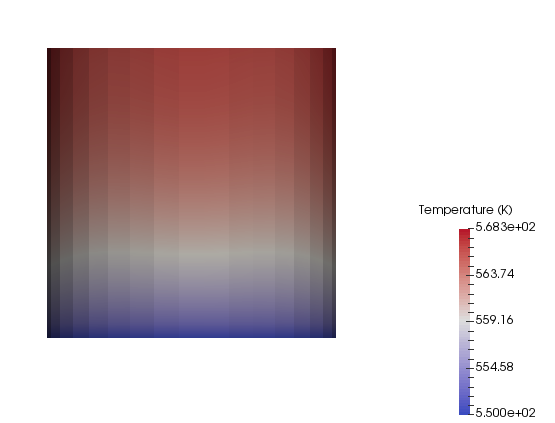
\includegraphics[width=0.8\linewidth]{../Figures/temp_right.png}
  \caption{Right side}
\end{subfigure}
\caption{Fuel temperature BC computed
on (a) the left and (b) right sides of the fuel pin.}
\label{fig:fuel_temps}
\end{figure}

Fig.~\ref{fig:layer_temps} shows the layer-averaged fluid temperatures
for several Picard iterations and the Nek5000 fluid temperature solution.
The fluid temperature increases moving up the pin,
as expected. Compared with Fig.~\ref{fig:k_avgtmp}(b), the fluid temperature
converges more slowly than the average fuel temperature and should also
be considered in more complex convergence criteria.

\begin{figure}[!htb]
\centering
\begin{subfigure}{.5\textwidth}
  \centering
  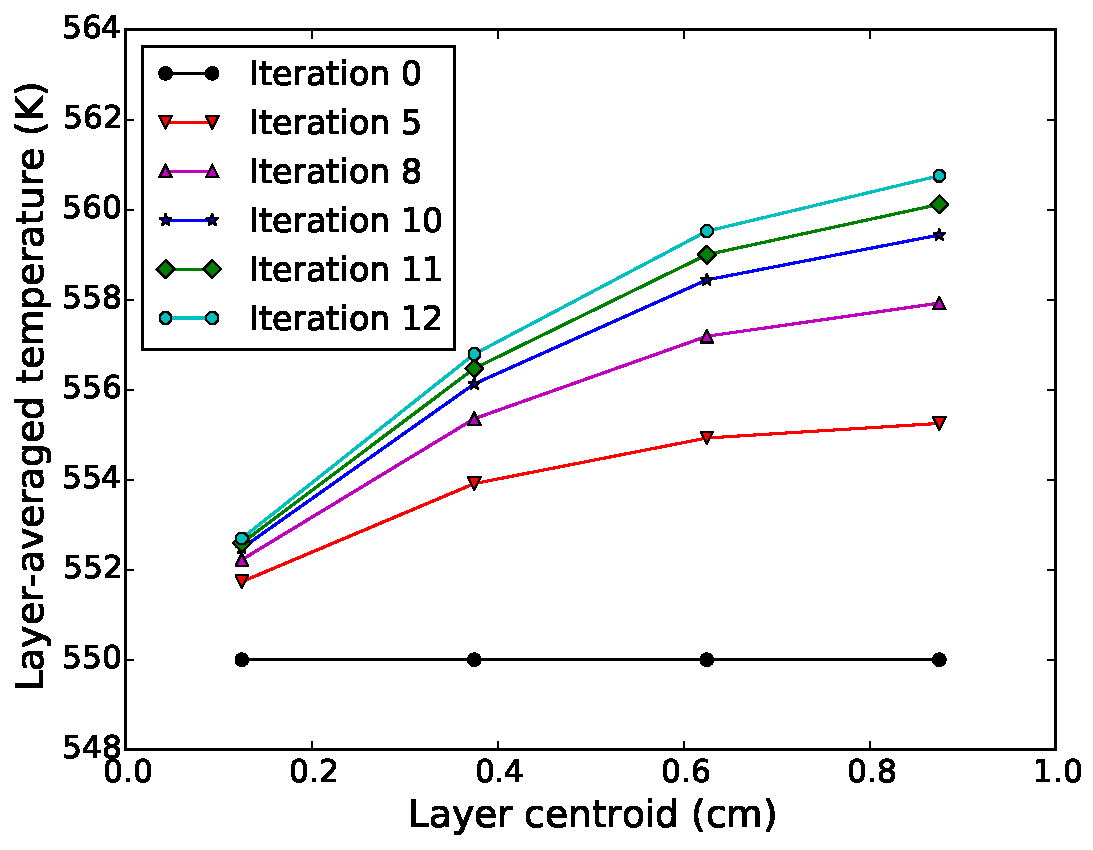
\includegraphics[width=0.8\linewidth]{../Figures/layer_temps.pdf}
  \caption{}
\end{subfigure}%
\begin{subfigure}{.5\textwidth}
  \centering
  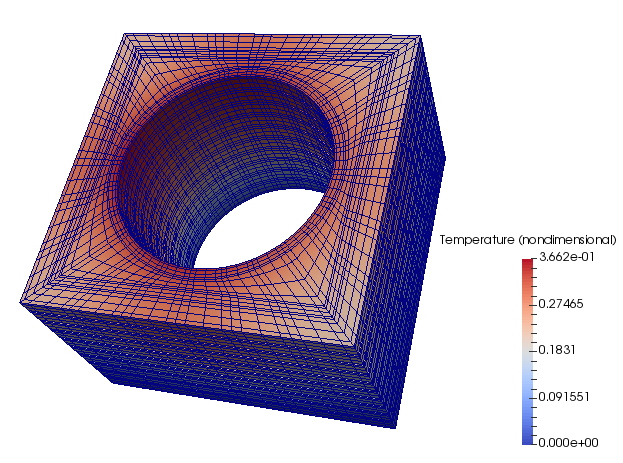
\includegraphics[width=0.8\linewidth]{../Figures/Nek_with_mesh.png}
  \caption{}
\end{subfigure}
\caption{(a) Layer-averaged fluid temperatures for several Picard iterations
and (b) fluid temperature at Picard iteration 12.}
\label{fig:layer_temps}
\end{figure}

\section{CONCLUSIONS}
\label{sec:Conclusions}
This paper presents a coupling of OpenMC and Nek5000
using the MOOSE framework. All data exchange occurs in-memory
using FEs such that only a few coefficients are needed to describe complex
spatial distributions. Results in this paper are shown for a three-way
coupling that includes Buffalo, a surrogate fuels simulation code, to demonstrate the potential for code reuse
with other MOOSE application couplings.
Preliminary results for a pincell problem demonstrate that the
Picard scheme converges to a steady-state solution within a reasonable
number of iterations. Results for fission distribution and temperatures
using the exaggerated radial asymmetry of the problem show the
interplay between the physics.

The work presented in this paper is preliminary, and many improvements
can be made to the coupling algorithm. Many aspects of the coupling have not yet
been optimized or investigated in detail, such as the choice of convergence criteria,
FE orders for the solution fields, and MC run strategy. Several researchers
have investigated methods to accelerate the Picard iteration,
and common strategies such as underrelaxation and partial convergence
of the fission source will be investigated. Improvements
may also be possible by implementing delta-tracking and using coarse
mesh finite difference acceleration to serve as an internal
thermal-hydraulics solver~\cite{Herman}. Use of some or all of
these techniques will be beneficial in furthering the development of
the general MC-CFD simulation capability available with the
OpenMC and Nek5000 coupling framework introduced here. With improvements over time, this
general modeling and simulation tool has the potential to provide reference solutions
for coupled simulations of complex reactor systems.


\section*{ACKNOWLEDGEMENTS}

% I have to say this part -
This work was made possible by a Nuclear Engineering University Programs
fellowship supporting the first author. This research was supported by the
Exascale Computing Project (17-SC-20-SC), a collaborative effort of the
U.S. Department of Energy (DOE) Office of Science and the National Nuclear Security
Administration. This material was based on work supported by the U.S. DOE, under
contract DE-ACO2-06CH11357.

% You can enter a bibliography into the document using the following format, or use the
% bibliography style file "physor.bst" found in the template directory.  You can use the bibliography style file
% by replacing the current bibliography block with:
% \setlength{\baselineskip}{12pt}
% \bibliographystyle{physor}
% \bibliography{physor}

\setlength{\baselineskip}{12pt}
\begin{thebibliography}{300}
\bibitem{Wu} X. Wu, and T. Kozlowski, ``Coupling of system thermal-hydraulics and
Monte-Carlo code: Convergence criteria and quantification of correlation between
statistical uncertainty and coupled error,'' \emph{Ann. Nucl. Energy},
  \textbf{75}, pp. 377--387 (2015).
\bibitem{Seker} V. Seker, J. Thomas, and T. Downar ,``Reactor simulation with
coupled Monte Carlo and computational fluid dynamics,''
\emph{Proceedings of M\&C},
  Monterey, California, April 15--19, 2007.
\bibitem{Cardoni} J. Cardoni, and R. Uddin, ``Nuclear reactor multi-physics simulations
with coupled MCNP5 and STAR-CCM+,'' \emph{Proceedings of ICONE},
  Rio de Janeiro, Brazil, May 8-12, 2011.
\bibitem{Breitkreutz} H. Breitkreutz, A. R{\"o}hrmoser, and W. Petry, ``3-dimensional
coupled neutronic and thermal-hydraulic calculations for a compact core
combining MCNPX and CFX,'' \emph{IEEE Transactions on Nuclear Science},
  \textbf{57}, pp. 3667--3671 (2010).
\bibitem{Sjenitzer} B. Sjenitzer, J. Hoogenboom, J. Escalante, and V. Espinoza,
``Coupling of dynamic Monte Carlo with thermal-hydraulic feedback,''
\emph{Ann. Nucl. Energy}, \textbf{76}, pp. 27--39 (2015).
\bibitem{Gurecky} W. Gurecky and E. Schneider, ``Development of an MCNP6-ANSYS FLUENT
multiphysics coupling capability,'' \emph{Proceedings of ICONE},
Charlotte, North Carolina, June 26--30, 2016.
%\bibitem{Li} L. Li, H. Yuan, and K. Wang
%``Coupling of RMC and CFX for analysis of pebble bed-advanced high temperature
%reactor core,'' \emph{Nucl. Eng. Des.}, \textbf{250}, pp. 385--391 (2012).
\bibitem{Ivanov} A. Ivanov, V. Sanchez, R. Stieglitz, and K. Ivanov,
``High fidelity simulation of conventional and innovative LWR with the coupled Monte-Carlo
thermal-hydraulic system MCNP-SUBCHANFLOW,''
\emph{Nucl. Eng. Des.}, \textbf{262}, pp. 264--275 (2013).
\bibitem{Daeubler} M. Daeubler, A. Ivanov, B. Sjenitzer, V. Sanchez, R. Stieglitz, and R. Macian-Juan,
``High-fidelity coupled Monte Carlo neutron transport and thermal-hydraulic
simulations using Serpent 2/SUBCHANFLOW,''
\emph{Ann. Nucl. Energy}, \textbf{83}, pp. 352--375 (2015).
\bibitem{Aufiero} M. Aufiero, C. Fiorina, A. Laureau, P. Rubiolo, and V. Valtavirta,
``Serpent-OpenFOAM coupling in transient mode: Simulation of a Godiva
prompt critical burst,'' \emph{Proceedings of M\&C},
Nashville, Tennessee, April 19--23, 2015.
\bibitem{Gill} D. Gill, D. Aumiller, and D. Griesheimer,
``Monte Carlo and thermal-hydraulic coupling via PVMEXEC,''
\emph{Proceedings of PHYSOR}, Kyoto, Japan, September 28-October 3, 2014.
\bibitem{Ellis} M. Ellis, D. Gaston, B. Forget, and K. Smith,
``Preliminary coupling of the Monte Carlo code OpenMC and the Multiphysics
Object-Oriented Simulation Environment for analyzing Doppler feedback in
Monte Carlo simulations,''
\emph{Nucl. Sci. Eng.}, \textbf{185}, pp. 184--193 (2017).
\bibitem{Romano} P. K. Romano, N. E. Horelik, B. R. Herman, A. G. Nelson, and B. Forget,
``OpenMC: A state-of-the-art Monte Carlo code for research and development,''
\emph{Ann. Nucl. Energy}, \textbf{82}, pp. 90--97 (2015)
\bibitem{Fischer} P. Fischer, J. Lottes, S. Kerkemeier, O. Marin, K. Heisey, et. al
``Nek5000: User's manual,''
Technical Report ANL/MCS-TM-351 (2015)
\bibitem{Gaston} D. Gaston, C. Permann, J. Peterson, A. Slaughter, D. Andr\v{s}, et. al,
``Physics-based multiscale coupling for full core nuclear reactor simulation,''
\emph{Ann. Nucl. Energy}, \textbf{84}, pp. 45--54 (2015)
\bibitem{Brown} F. Brown and W. Martin,
``Direct sampling of Monte Carlo flight paths in media with continuously
varying cross-sections,''
\emph{Proceedings of Nuclear Mathematical and Computational Sciences},
Gatlinburg, Tennessee, April 6--11, 2003.
\bibitem{Wendt} B. Wendt, A. Novak, L. Kerby, and P. Romano, ``Integration of
  functional expansion methodologies as a MOOSE module,'' \emph{Proceedings of
    PHYSOR}, Cancun, Mexico, April 22--26, 2018.
\bibitem{Leppanen} J. Lepp{\"a}nen, V. Valtavirta, T. Viitanen, and M. Aufiero,
``Unstructured mesh based multi-physics interface for CFD code coupling
in the Serpent 2 Monte Carlo code,''
\emph{Proceedings of PHYSOR}, Kyoto, Japan, September 28-October 3, 2014.
\bibitem{Kerby} L. Kerby, A. Tumulak, J. Lepp{\"a}nen, and V. Valtavirta,
``Preliminary Serpent-MOOSE coupling and implementation of functional
expansion tallies in Serpent,''
\emph{Proceedings of M\&C},
Jeju, Korea, April 16--20, 2017.
\bibitem{Herman} B. Herman, B. Forget, and K. Smith,
``Progress toward Monte Carlo-thermal hydraulic coupling using
low-order nonlinear diffusion acceleration methods''
\emph{Ann. Nucl. Energy}, \textbf{84}, pp. 63--72 (2015)
\end{thebibliography}

\end{document}
